\documentclass[tikz,border=5]{standalone}
\usepackage{physics}
\usepackage{tikz}
\usetikzlibrary{angles,quotes} % for angle label
\usetikzlibrary{bending} % for arrow head angle
\tikzset{>=latex} % for LaTeX arrow head

\colorlet{myred}{red!65!black}
\colorlet{metalcol}{blue!25!black!30!white}
\tikzstyle{mass}=[line width=0.6,red!30!black,fill=red!40!black!10,rounded corners=1,
                  top color=red!40!black!20,bottom color=red!40!black!10,shading angle=20]
\tikzstyle{rod}=[line width=0.5,red!30!black,fill=red!40!black!30,rounded corners=1,
                  top color=red!40!black!60,bottom color=red!40!black!30,shading angle=90]

\begin{document}


% INCLINED ground
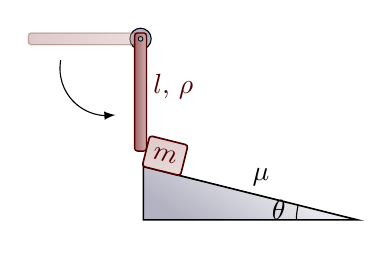
\begin{tikzpicture}
  \def\height{0.4}  % mass height
  \def\width{0.5}  % mass width
  \def\rLength{1.5}  % rod length
  \def\rThickness{0.15} % rod thickness
  \def\gWidth{2.8}  % inclined ground width
  \def\gAng{14} % inclined ground angle
  \coordinate (R) at ({\gWidth*cos(\gAng)},0); % right corner inclined ground
  \coordinate (L) at (0,0);              % left corner inclined ground
  \coordinate (T) at (0,{\gWidth*sin(\gAng)}); % top inclined ground
  \coordinate (P) at ({-\rThickness/2+0.33*\width*sin(\gAng)},{\gWidth*sin(\gAng)+\rLength+0.25*\width*cos(\gAng)}); % rod pivot point
  
  % ROD
  \draw[fill=metalcol] (P) circle(0.9*\rThickness);
  \draw[rod,opacity=0.25] (P)++(\rThickness/2,\rThickness/2) rectangle++ (-\rLength,-\rThickness);
  \draw[rod] (P)++(-\rThickness/2,\rThickness/2) rectangle++ (\rThickness,-\rLength)
    node[midway,above=2,right=1] {$l$, $\rho$}; %\ell
  \draw[fill=metalcol,line width=0.3] (P) circle(0.03);
  \draw[->] (P)++(195:0.7*\rLength) arc(170:280:0.4*\rLength);
  
  % MASS ON INCLINED GROUND
  \draw[line width=0.6,top color=blue!20!black!30,bottom color=white,shading angle=160-\gAng]
    (L) -- (T) -- (R) node[pos=0.55,above] {$\mu$} -- cycle;
  \draw[mass,rotate=-\gAng] (-0.03*\width,0)++(90+\gAng:{\gWidth*sin(\gAng)}) rectangle++ (\width,\height) node[midway,rotate=-\gAng] {$m$};
  \draw pic["$\theta$",draw=black,angle radius=22,angle eccentricity=1.3] {angle=T--R--L};
  
\end{tikzpicture}



\end{document}